\documentclass[12pt, a4paper]{article}

\usepackage[czech]{babel}
\usepackage{lmodern}
\usepackage[utf8]{inputenc}
\usepackage[T1]{fontenc}
\usepackage[pdftex]{graphicx}
\usepackage{amsmath, amssymb}
\usepackage[hidelinks,unicode]{hyperref}
\usepackage{float}
\usepackage{listings}
\usepackage{tikz}
\usepackage{xcolor}
\usepackage{tabularx}
\usepackage[final]{pdfpages}
\usepackage{syntax}
\usepackage{caption}
\usepackage{subcaption}
\usepackage{amsfonts}
\usepackage{siunitx}


\definecolor{mauve}{rgb}{0.58,0,0.82}
\usetikzlibrary{shapes,positioning,matrix,arrows}

\newcommand{\img}[1]{(viz obr. \ref{#1})}

\definecolor{pblue}{rgb}{0.13,0.13,1}
\definecolor{pgreen}{rgb}{0,0.5,0}
\definecolor{pred}{rgb}{0.9,0,0}
\definecolor{pgrey}{rgb}{0.46,0.45,0.48}


\lstdefinestyle{flex}{
    frame=tb,
    aboveskip=3mm,
    belowskip=3mm,
    showstringspaces=false,
    columns=flexible,
    basicstyle={\small\ttfamily},
    numbers=none,
    numberstyle=\tiny\color{black},
    keywordstyle=\color{black},
    commentstyle=\color{black},
    stringstyle=\color{black},
    breaklines=true,
    breakatwhitespace=true,
    tabsize=3
}

\lstset{
    frame=tb,
    language=Python,
    aboveskip=3mm,
    belowskip=3mm,
    showstringspaces=false,
    columns=flexible,
    basicstyle={\small\ttfamily},
    numbers=none,
    numberstyle=\tiny\color{gray},
    keywordstyle=\color{blue},
    commentstyle=\color{pgreen},
    stringstyle=\color{mauve},
    breaklines=true,
    breakatwhitespace=true,
    tabsize=3
}


\let\oldsection\section
\renewcommand\section{\clearpage\oldsection}

\begin{document}
	% this has to be placed here, after document has been created
	% \counterwithout{lstlisting}{chapter}
	\renewcommand{\lstlistingname}{Ukázka kódu}
	\renewcommand{\lstlistlistingname}{Seznam ukázek kódu}
    \begin{titlepage}

        \centering

        \vspace*{\baselineskip}
        \begin{figure}[H]
        \centering
        
\includegraphics[width=7cm]{img/fav-logo.jpg}
        \end{figure}

        \vspace*{1\baselineskip}

        \vspace{0.75\baselineskip}

        \vspace{0.5\baselineskip}
        {Domácí úkol z předmětu KIV/VSS}

        {\LARGE\sc Sítě front\\}

        \vspace{4\baselineskip}

        \vspace{0.5\baselineskip}

        {\sc\Large Stanislav Král \\}
        \vspace{0.5\baselineskip}
        {A20N0091P}

        \vfill

        {\sc Západočeská univerzita v Plzni\\
        Fakulta aplikovaných věd}

    \end{titlepage}

    % TOC
    \tableofcontents
    \pagebreak

\section{Zadání}
Pro zadanou otevřenou síť front vypočítejte odhad hodnot $L_q$ a $T_q$.
Časové intervaly mezi vstupy požadavků mají exponenciální rozdělení s parametrem $\lambda = 0.5$, oba kanály obsluhy mají gaussovsky rozdělenou dobu obsluhy se středními hodnotami $T_{s1} = 1$, $T_{s2} = 1.33$ (směrodatné odchylky si zvolte dle svého uvážení, ideálně aby pak koeficient variace byl kolem 0.5).

\begin{figure}[!ht]
    \centering
    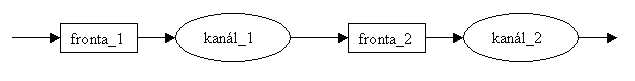
\includegraphics[width=.95\linewidth]{img/assignment.jpg}
    \label{fig:}
\end{figure}

\noindent Dále určete střední frekvenci výstupního toku požadavků.

\section{Vypracování}

Nejprve si zvolíme směrodatné odchylky doby obsluhy tak, aby koeficient variace byl zhruba 0.5 (dle zadání):

\begin{equation}
    \begin{split}
    & \sigma_{s1} = 0.5 \\
    & C_{s1} =  \frac{\sigma_{s1}}{T_{s1}} = \frac{0.5}{1} = 0.5 \\
    & \\
    & \sigma_{s2} = 0.665 \\
    & C_{s2} =  \frac{\sigma_{s2}}{T_{s2}} = \frac{0.665}{1.33} = 0.5 \\
    \end{split}
\end{equation}

Poté vypočteme vnitřní frekvence toků v uzlech:

\begin{figure}[!ht]
    \centering
    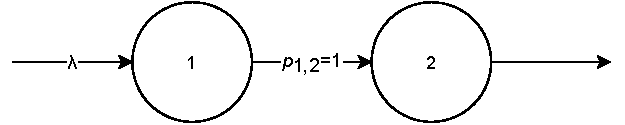
\includegraphics[width=.65\linewidth]{pdf/flow-diagram.pdf}
    \label{fig:flowdiagram}
\end{figure}

\begin{equation}
    \begin{split}
    & \Lambda_{1} = 0.5 \\
    & \Lambda_{2} = p_{1,2}\Lambda_1 = 1 \cdot 0.5 = 0.5 \\
    \end{split}
\end{equation}

Uzly jsou stacionární, protože jejich zatížení jsou menší než 1:

\begin{equation}
    \begin{split}
    & \rho_1 = \Lambda_1T_1 = 0.5 \cdot 1 = 0.5 \\
    & \rho_2 = \Lambda_2T_2 = 0.5 \cdot 1.33 = 0.665 \\
    \end{split}
\end{equation}

Dále vypočítáme střední doby $L_{q1}$ a $L_{q2}$ tak, že odvodíme obecné $L_q$ z $L_w$ pro Kendellovu klasifikaci \textit{M/G/1}, které odpovídá popis zadání:


\begin{equation}
    \begin{split}
    & L_w = L_{w(M/M/1)} \frac{1+C_{s}^{2}}{2} = \frac{\rho^2}{1 - \rho} \frac{1+C_{s}^{2}}{2}\\
    & L_q = L_w + \rho =  \frac{\rho^2}{1 - \rho} \frac{1+C_{s}^{2}}{2}  + \rho \\
    & L_{q_1} = \frac{0.5^2}{1 - 0.5} \frac{1+0.5^{2}}{2} + 0.5 = 0.8125 \\
    & L_{q_2} = \frac{0.665^2}{1 - 0.665} \frac{1+0.5^{2}}{2} + 0.665 \doteq 1.49 \\
    \end{split}
\end{equation}

$L_q$ celého systému lze vypočítat jako součet $L_{q_1}$ a $L_{q2}$:



\begin{equation}
    \begin{split}
    & L_q = L_{q1} + L_{q2} = 0.8125 + 1.49 \doteq 2.3025 \\
    \end{split}
\end{equation}

$T_q$ nakonec spočítáme ze vzorce $T_q$ pro klasifikaci \textit{M/G/1}:

\begin{equation}
    \begin{split}
    & T_q = \frac{L_q}{\lambda} = \frac{2.3025}{0.5} \doteq 4.6051 \\
    \end{split}
\end{equation}

Frekvence výstupního toku sítě je převrácená hodnota střední doby obsluhy druhého (posledního) uzlu:

\begin{equation}
    \begin{split}
    & \mu = \frac{1}{T_{s_2}} = \frac{1}{1.33} \doteq \SI[product-units = single]{0.7519}{\Hz} \\
    \end{split}
\end{equation}


\end{document}

